\documentclass[a4paper]{article}
\usepackage[
				pdftex,
				colorlinks=true,
				bookmarksnumbered=true,
				bookmarksopen=true,
				bookmarksopenlevel=3,
				pdfstartview=FitP,
				urlcolor=blue,
			]{hyperref}
\pdfinfo{
			/Title(Esercitazione di Laboratorio: Arduino)
			/Author(Coa Giulio, Licastro Dario, Montano Alessandra)
		}
\usepackage[italian]{babel}
\usepackage{geometry,titling,mdsymbol,stmaryrd,graphicx,subcaption,amsmath}
\graphicspath{{./Image/}}
\renewcommand\maketitlehooka{
								\null
								\mbox{}
								\vfill
							}
\renewcommand\maketitlehookd{
								\vfill
								\null
							}
\title{
		\begin{center}
			Esercitazione di Laboratorio:
		\end{center}
		\newline
		\begin{center}
			Arduino
		\end{center}
	}
\author{
	Coa Giulio (s236723)
	\and
	Licastro Dario (s234421)
	\and
	Montano Alessandra (s238160)
}
\begin{document}
	%-----------------------------------------------------------------------------
	%  TITLE
	%-----------------------------------------------------------------------------
	\begin{titlingpage}
		\maketitle
	\end{titlingpage}
	\newpage
	%-----------------------------------------------------------------------------
	%  PURPOSE OF THE EXPERIENCE
	%-----------------------------------------------------------------------------
	\section{Scopo dell'esperienza}
		Lo scopo di questa esercitazione è sviluppare un termometro digitale tramite l'uso di un sensore di temperatura e di una scheda Arduino.
	%-----------------------------------------------------------------------------
	%  INSTRUMENTATION USED
	%-----------------------------------------------------------------------------
	\section{Strumentazione utilizzata}
		La strumentazione usata durante l'esercitazione è:
		\begin{center}
			\begin{tabular}{ |c|c|c| }
				\hline
				\multirow{\textbf{Strumento}}	 		   & \textbf{Marca e Modello} & \textbf{Caratteristiche} \\
				\hline
				\multirow{Multimetro}			 		   & Agilent 34401A			  & \\
				\multirow{Oscilloscopio}		 		   & Rigol DS1054Z			  & 4 canali, \\
												 		   &						  & $ B = 50 \, \mathrm{MHz} $, \\
												 		   &						  & $ f_{\mathrm{c}} = 1 \, \mathrm{G\frac{Sa}{s}} $, \\
												 		   &						  & $ R_{\mathrm{i}} = 1 \, \mathrm{M\Omega} $, \\
												 		   &						  & $ C_{\mathrm{i}} = 13 \, \mathrm{pF} $, \\
												 		   &						  & $ 12 \, \mathrm{Mbps} $ di profondità di memoria \\
				\multirow{Generatore di segnali} 		   & Rigol DG1022			  & 2 canali, \\
												 		   &						  & $ f_{\mathrm{uscita}} = 20 \, \mathrm{MHz} $, \\
												 		   &						  & $ Z_{\mathrm{uscita}} = 50 \, \mathrm{\Omega} $ \\
				\multirow{Scheda Arduino}	 		   	   & UNO					  & $ f_{\mathrm{c, max}} = 76.9 \, \mathrm{k\frac{Sa}{s}} $ \\
				\multirow{Sensore di temperatura}	 	   & LM335					  & $ S = 10 \, \mathrm{m\frac{V}{K}} $, \\
														   &						  & $ V_{\mathrm{out}} = 0 \, \mathrm{V} $ @ $ 0 \, \mathrm{K} $ \\
														   &						  & $ \delta T = \pm 1 \, $ \textdegree $ \mathrm{C} $ @ $ 25 \, $ \textdegree $ \mathrm{C} $ \\
				\multirow{Cavi coassiali}		 		   &						  & Capacità dell'ordine dei $ 80 \div 100 \, \mathrm{p\frac{F}{m}} $ \\
				\multirow{Connettori}			 		   &						  & \\
				\hline
			\end{tabular}
		\end{center}
	%-----------------------------------------------------------------------------
	%  THEORETICAL PREMISES
	%-----------------------------------------------------------------------------
	\section{Premesse teoriche}
		\subsection{Incertezza sulla misura dell'oscilloscopio}
			La misura del valore di un segnale tramite l’oscilloscopio (sia esso l'ampiezza, la frequenza, il periodo, etc.) presenta un'incertezza che dipende, principalmente, da due fattori:
			\begin{itemize}
				\item l’incertezza strumentale introdotta dall’oscilloscopio (ricavabile dal manuale).
				\item l’incertezza di lettura dovuta all’errore del posizionamento dei cursori.
			\end{itemize}
			Quest’ultima incertezza deriva dal fatto che il segnale visualizzato non ha uno spessore nullo sullo schermo.
		\subsection{Arduino}
			Arduino è una piattaforma elettronica open surce basata su un hardware di facile utilizzo e programmabie in un ambiente software dedicato.
			\subsubsection{Arduino UNO}
				Arduino UNO è una scheda composta da un convertitore ADC a $ 10 $ bit ($ 8 $ bit se la frequenza d'utilizzo è maggiore di $ 15 \, \mathrm{k\frac{Sa}{s}} $) che può essere alimentato da due distinte sorgenti, una interna alla scheda da $ 1.1 \pm 0.1 \, \mathrm{V} $ e una esterna da $ 5 \pm 0.25 \, \mathrm{V} $ ($ 4.85 \pm 0.4 \, \mathrm{V} $ se si usa la porta USB 3.0 anzichè la porta USB 2.0).
				\begin{figure}[h!]
					\centering
					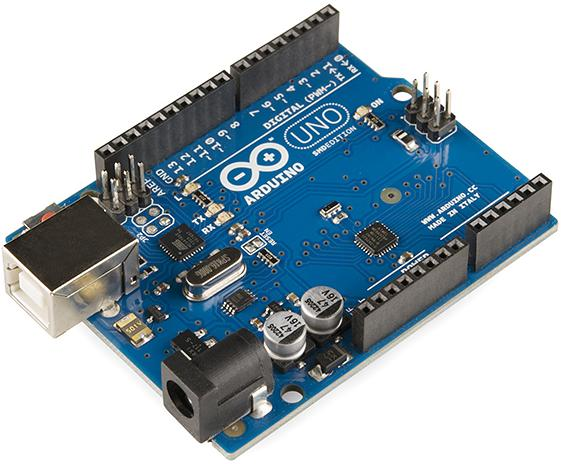
\includegraphics[scale=0.6]{ArduinoUNO}
					\caption{Arduino UNO.}
					\label{fig:ArduinoUNO}
				\end{figure}
		\subsection{Sensore LM335}
			Il sensore LM335 è un sensore di temperatura prodotto dalla National Semiconductor; esso permette di avere in uscita una tensione proporzionale alla temperatura rilevata ($ V_{\mathrm{out}} = S \cdot T_{\mathrm{K}} $).
			\newline
			Il suo comportamento è assimilabile a quello di un diodo di Zener la cui corrente $ I_{\mathrm{d}} $ deve essere compresa nell'intervallo $ 0.4 \, \mathrm{mA} \div 5 \, \mathrm{mA} $.
			\begin{figure}[h!]
				\centering
				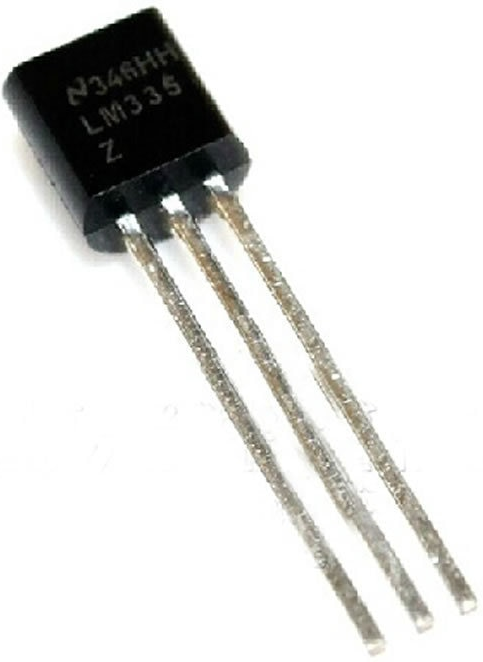
\includegraphics[scale=0.2]{LM335}
				\caption{Sensore LM335.}
				\label{fig:LM335}
			\end{figure}
		\subsection{Other}
			.
	%-----------------------------------------------------------------------------
	%  LABORATORY EXPERIENCE
	%-----------------------------------------------------------------------------
	\section{Esperienza in laboratorio}
		\subsection{Other}
			.
	%-----------------------------------------------------------------------------
	%  RESULTS
	%-----------------------------------------------------------------------------
	\section{Risultati}
		\subsection{Other}
			.
\end{document}